\chapter{Testy modułu}
	Do lepszego zrozumienia oraz wykorzystania nowo powstałej biblioteki warto znać jej lepsze oraz słabsze strony, a także teoretyczne i praktyczne ograniczenia. W związku z tym przeprowadzone zostały testy różnych aspektów omawianego projektu, aby ustalić limity ilościowe i wydajnościowe, a także ich przyczyny w celu opracowania możliwości ich poprawy.
	
	\section{Framework testowy}
	Do łatwiejszego tworzenia testów utworzona został utworzony interfejs - \textbf{ITest}, która ujednolica API testów do późniejszego wykorzystania. Obiekty dziedziczące implementują metody \textit{Init()} do inicjalizacji oraz \textit{Update()} do aktualizacji co klatkę obrazu.
	
	Podzbiorem testów są także pomiary wydajności i/lub limitu ilości testowanego parametru. Do obsługi tego zbioru oddana została druga klasa - \textbf{AutoTest}. Dziedziczy ona z \textit{ITest}, ale nadpisuje \textit{Init()} i \textit{Update()} własnymi funkcjami. Udostępnia zamiast tego własny interfejs opisany w dalszej części rozdziału. Różnicą względem rodzica jest próba automatycznego dopasowania złożoności testu do założonego poziomu wydajności. 
	
	\subsection{Metoda określania wydajności przez AutoTest}
	Każdy oparty o \textit{AutoTest} skrypt musi posiadać wartość mierzalną, nazwaną w uproszczeniu ilością (\textit{count}). Zwiększenie tej wartości powinno z założenia liniowo zmniejszać wydajność renderowania, a co za tym idzie zwiększać czas generowania klatki obrazu. Informacja o długości rysowania jest następnie agregowana przez 100 wpisów przy pomocy obiektu klasy \textbf{AverageAccumulator} do wartości średniej, która zostaje przyrównana z czasem oczekiwanym, definiowanym przez test za pomocą metody \textit{GetTargetFPS()}. Na podstawie wzajemnej proporcji tych wartości obliczana jest teoretyczna ilość potrzebnych do dodania elementów, aby osiągnąć zamierzony cel. Przed zwiększeniem ilości mierzalnej za pomocą funkcji \textit{IncreaseCount()}, rozmiar zwiększenia zostaje pomniejszony przez pomnożenie o wartość z wirtualnej metody \textit{GetTargetCurveMultiplier()}, co ma na celu zmniejszenie prawdopodobieństwa przeszacowania celu. Cykl ten powtarzany jest aż do zejścia czasu rysowania klatki poniżej progu. Następnym krokiem jest stopniowa powtarzanie operacji, ale zmniejszając ilość o 1 za pomocą \textit{DecreaseCount()} zamiast zwiększać, aż do ponownego przekroczenia docelowej długości renderowania w trzech bezpośrednio następujących po sobie pomiarach. Taka forma pomiaru pozwala na powtarzalne określenie maksymalnej ilości elementów spełniających założony cel wydajnościowy. Wykres czasu klatki z przykładowego testu oświetlenia został przedstawiony w całości na rys. \ref{Test_LightsTest_FullFrameTime} oraz ograniczony do partii autoregulacji na rys. \ref{Test_LightsTest_AutoFrameTime}.
	
	\begin{figure}[h!]
\begin{center}
		\begin{subfigure}{.45\textwidth}
			\centering
			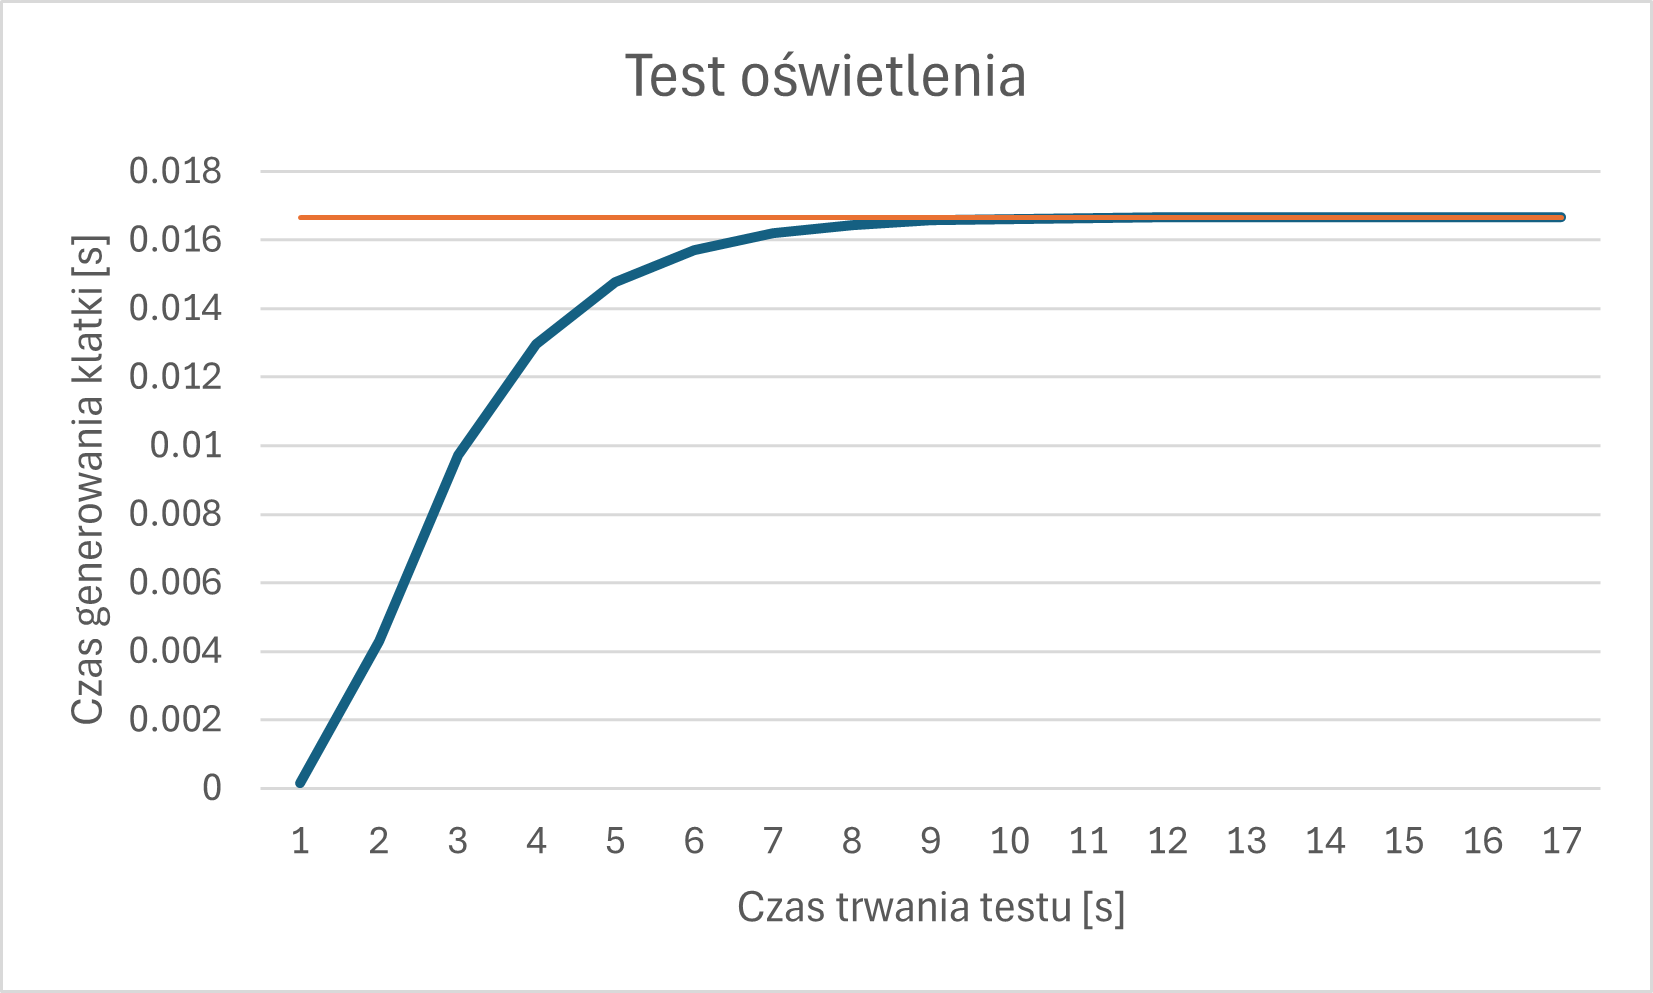
\includegraphics[width=\textwidth]{images/LightsTestResult_full.png}
			\caption{Pełny wykres czasu generowania klatki.}
			\label{Test_LightsTest_FullFrameTime}
		\end{subfigure}
		\begin{subfigure}{.45\textwidth}
			\centering
			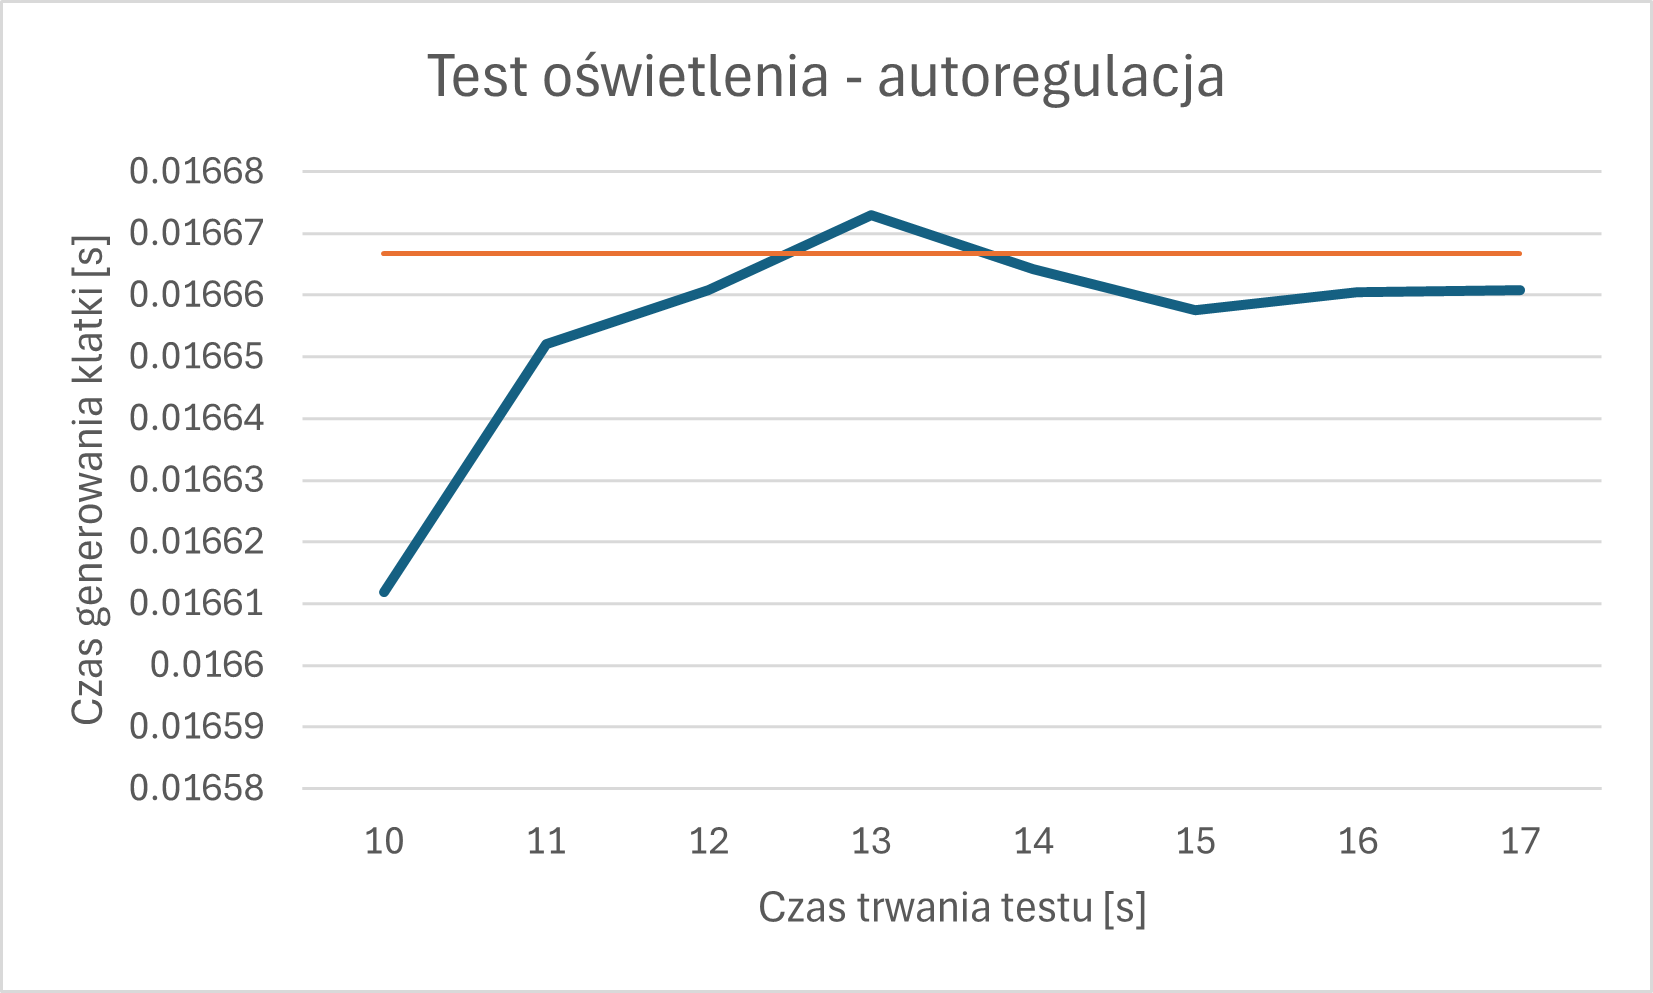
\includegraphics[width=\textwidth]{images/LightsTestResult_auto.png}
			\caption{Czas rysowania obrazu dla fragmentu autoregulacji.}
			\label{Test_LightsTest_AutoFrameTime}
		\end{subfigure}
		\caption{Wykres pokazujący działanie mechanizmu \textit{AutoTest} podczas testu oświetlenia.}
\end{center}
	\end{figure}
	
	\subsection{Eliminacja błędów}
	Aby test był wiarygodny należy zabezpieczyć go na wypadek wystąpienia różnego rodzaju błędów. Poniżej przedstawiona została lista potencjalnych problemów oraz podjęte działania w celu ich eliminacji.
	\begin{itemize}
		\item \textbf{Anomalie pomiaru} - generowanie klatek obrazu nie zawsze odbywa się całkowicie stabilnie. Skokowe obciążenie systemu procesem w tle, nieprzewidziane zwalnianie zasobów przez system operacyjny, a nawet błędy sprzętowe mogą powodować skok czasu generowania pojedynczych klatek obrazu. Takie pomiary eliminowane są przy pomocy algorytmu IQR, służącego do wykrywania anomalii, w tym przypadku przyjmujących formę czasu wyraźnie odbiegającego od pozostałych pomiarów. Taki sposób filtracji jest możliwy ze względu na obraną metodę, gdyż w idealnych warunkach powinna ona generować niezmienną wartość pomiarów pomiędzy zmianami ilości.
		\item \textbf{Wpływ dodawania elementów na czas generowania klatki} - alokacja i inicjalizacja dużej ilości obiektów może generować wyraźne skoki czasu renderowania klatki obrazu. Zostały zaimplementowane dwa mechanizmy mające na celu zapobieganie takim sytuacjom. Pierwszym jest opisany już IQR, który powinien eliminować wyraźne anomalie. Drugi to zatrzymanie czasomierza w \textit{AverageAccumulator} na czas przetwarzania wyników pomiarów - w tym ewentualne zwiększenie bądź zmniejszenie ilości elementów - a następne wznowienie już po wykonaniu opisanych czynności. 
		\item \textbf{Przeszacowanie zwiększenia ilości elementów} - mechanizm odpowiedzialny za ograniczenie takiej sytuacji został już opisany - najpierw szacunkowo zostaje określone zwiększenie wartości mierzalnej powodujące spadek wydajności poniżej progu, aby potem bardzo powolną redukcją nastąpiło określenie wartości docelowej. Dodatkowym sposobem jest nadpisywalna metoda \textit{GetTargetCurveMultiplier()}, dzięki której bardziej złożone testy mogą zmniejszyć prawdopodobieństwo przeszacowania, kosztem zwiększonego czasu trwania testu.
		\item \textbf{Niedokładność czasu pomiaru} - użycie klasy \textit{high\_resolution\_clock} ze standardowej biblioteki C++ umożliwia dokonywanie pomiaru czasu z bardzo wysoką precyzją liczoną w nanosekundach.
	\end{itemize}